\section{Neural Network background theory}
In this section, the basis and the theoretical background of the convolutional neural networks theory is exposed.\\

\subsection{Historical introduction}
The historical introduction to neural networks is going to be summarized \cite{BINN}:\\

Neural Networks are introduced by first time in the years 40 by Warren McCulloch and Walter Pitts, more specifically, simple models of neural networks (switches based on neurons) were able to calculate almost every arithmetic problems and logic operations. Few years layer, the recognition of spacial patterns field was defined as a interesting scope for neural networks.\\

In 1949 the `Hebbian rule' was postulate by Donald O. Hebb. The rules describes the generalized learning basis of neural networks. This rule explain that two connected neurons have  a bigger strength if they are active at the same time, and the strength changes proportionally to the product of the two activities.\\

From 1951, the golden age of neural networks start although it stopped with a big pause. The first neurocomputer which was capable to adjust the weights by itself was developed in 1951 and was called \textit{Snark}. The fist neurocomputer able to recognize simple numbers was called \textit{`Mark I perceptron'} as was developed between 1957 and 1958.\\

It was in 1959 when Franck Rosenblatt  defined the \textit{perceptron} and the \textit{perceptron convergence theorem} was verified. One year later, the \textit{ADALINE (ADAptive LInear NEuron)} was developed, this was the first commercially used neural network which was a fast and precise system. One important characteristic was the \textit{delta rule} rule used for the training procedure. Before the golden age finished, researched figured out that the XOR function was not able to be solve with just one perceptron.\\

From these years, neural networks does not have much importance, until computational resources were enough. But some important advances were developed ad the \textit{linear associator} model (an associative memory model). The backpropagation of error, a very used learning procedure was defined in 1974 by Paul Werbos. \textit{The self-organizing feature maps} were described in 1982, there are also known as Kohonen maps. In 1983, a neural model able to recognize handwritten characters was developed as an extension of the Cognitron, the new model was called Neocognitron.\\

From this time on, neural networks are having a significant importance and are researched widely, it has to notice, that nowadays the computational resources are bigger than some years and that makes that the researchers could be more extensive.\\

\subsection{Introduction to ANN}
Humans, along the history, have tried to reproduce nature. Evolution, has turned out to be a big coordination in nature. If object recognition, associate concepts, memorize or extracting the semantic of images are focused, humans are provided of those processing information qualities. Trying to get those qualities with technology is a current (and not surprising) challenge.\\

One of the matters that is increasing its importance are neural networks which are inspired in biological neural networks. Neural networks are a important subject of the Artificial Intelligence (AI) and it is a new way (and more sophisticated) of processing information \cite{Rojas}.\\

\subsection{Biological Neural Networks}
Biological neural networks are part of the nervous system and are formed by neurons units or nervous cells. Each neuron is a capable of process information in different ways by itself \cite{Rojas}.\\

\begin{figure}[htb]
\centering
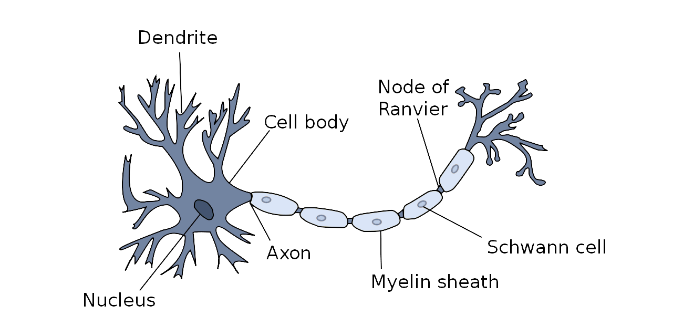
\includegraphics[width=0.65\textwidth]{images_miscelaneus/neuron.png}
\caption{Biological Neural Network. Image obtained from \cite{BINN}} \label{fig:Bio-Neuron}
\end{figure}


The principal components of a neuron are the nucleus, dendrite, cell body, axon, schwann cell, the node of Ranvier... In figure \ref{fig:Bio-Neuron} a biologica neural is shown in which its components are signalized \cite{BINN}.\\

The soma is the spherical central part of the nerve cell in whose there is a salt and potassium concentration which is covered by the neuronal membrane. Inside the soma is the neuronal nucleus and from the soma branches are extend (dendrites). Nerve cells are connected among them by dendrites. Neurons are transmitting and receiving nervous signals continuously, communicating among them. The information transference is produced, more specifically, in the synaptic clef (space between two neurons connection). This exchange of information is denominated synapses and it is made though electrochemical activities. The axon is a soma extension whose responsibility is transmitting the information electrochemical out of the neuron, by the nervous system thanks to its terminal branches \cite{BINN, neuroscience}\\

\subsection{Artificial Neural Networks (ANN)}
As the same way as the nervous systems is formed by neurons, artificial neural networks are composed by artificial neurons. Each artificial neuron is a processing unit whose input is processed and shared to another neuron or to the output. Neurons are connected among them \cite{BINN}\\

Basically, there are three types of artificial neurons:
\begin{description}[noitemsep,topsep=8pt,parsep=0pt,partopsep=20pt]
\item \textbf{Input neurons}, if belong to the input layer. This neurons receive the input data of the network.
\item \textbf{Hidden Units}, if belong to the processing layers. There are many types of layers: convolutional, pooling, dropout... There could be as many hidden layers and hidden units as user desire. The connectivity and the topology of the layers define the topology of the network.
\item \textbf{Output neurons}, if belong to the output layer. This neurons gives the user the processed information.
\end{description}

In figure \ref{fig:esquemaneuronal} the schematic of a general neural network it is possible to visualize the schematic of a general neural network with an undefined number of neurons in each layer and an undefined number of hidden layers.\\

\begin{figure}[htb]
\centering
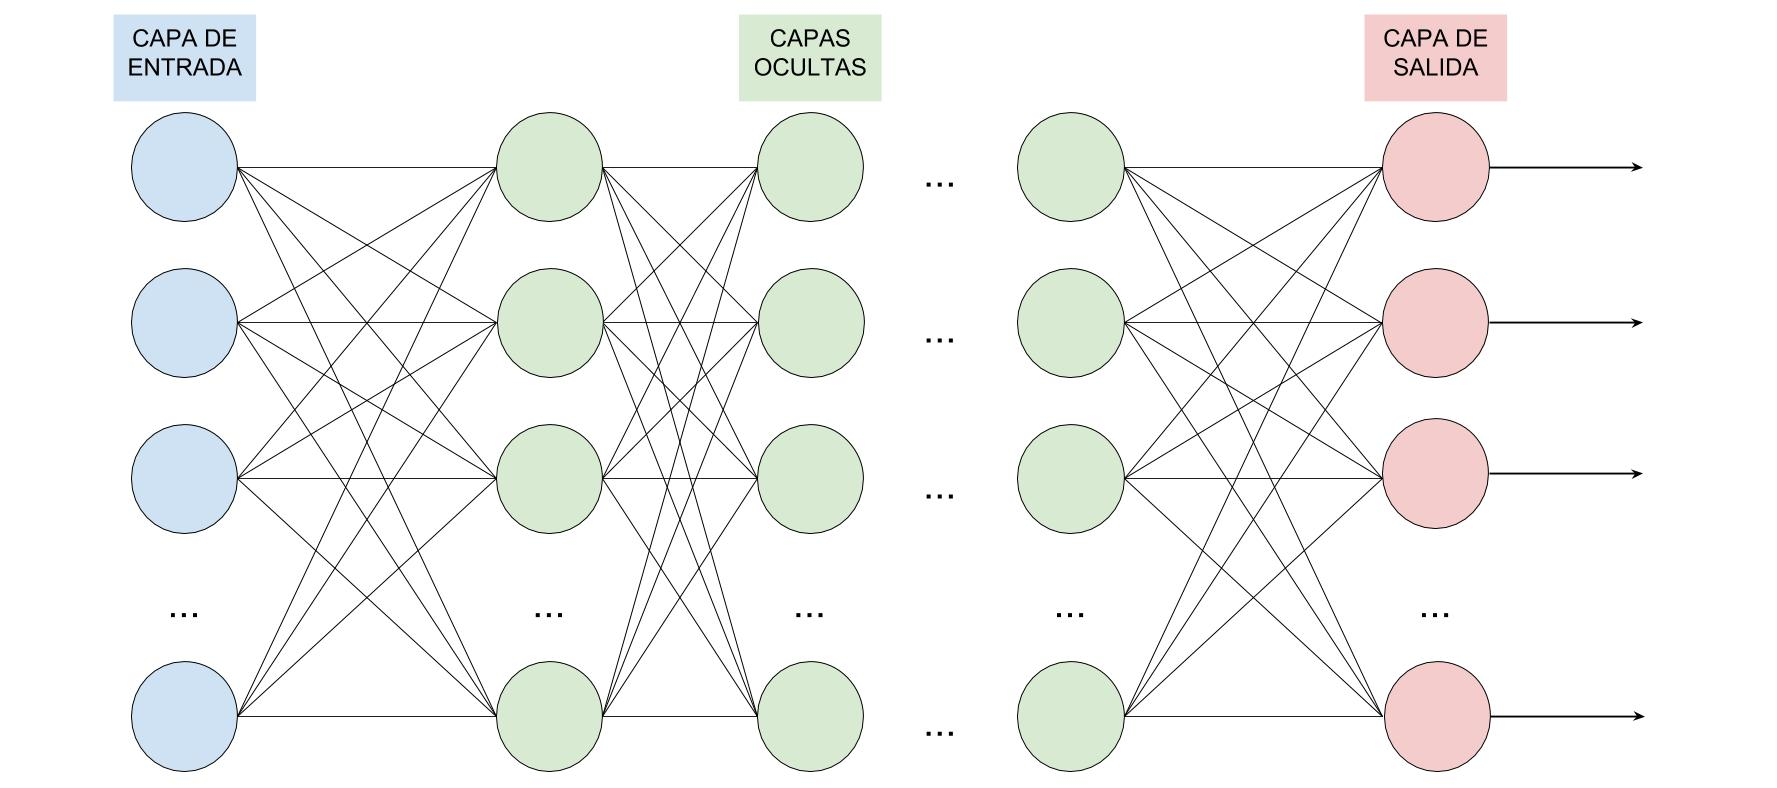
\includegraphics[width=0.55\textwidth]{images_miscelaneus/red_neuronal.jpg}
\caption{Schematic of a general neural network.} \label{fig:esquemaneuronal}
\end{figure}

A single neuron is formed by an input, a weight \textit{W} and a bias \textit{b} associated (Independent term). The value of the bias is always 1, but it has an associated weight that make that the value of the bias change. Weight and bias values could be modified. The output of the neuron is associated to an activation function. \\

\begin{figure}[htb]
\centering
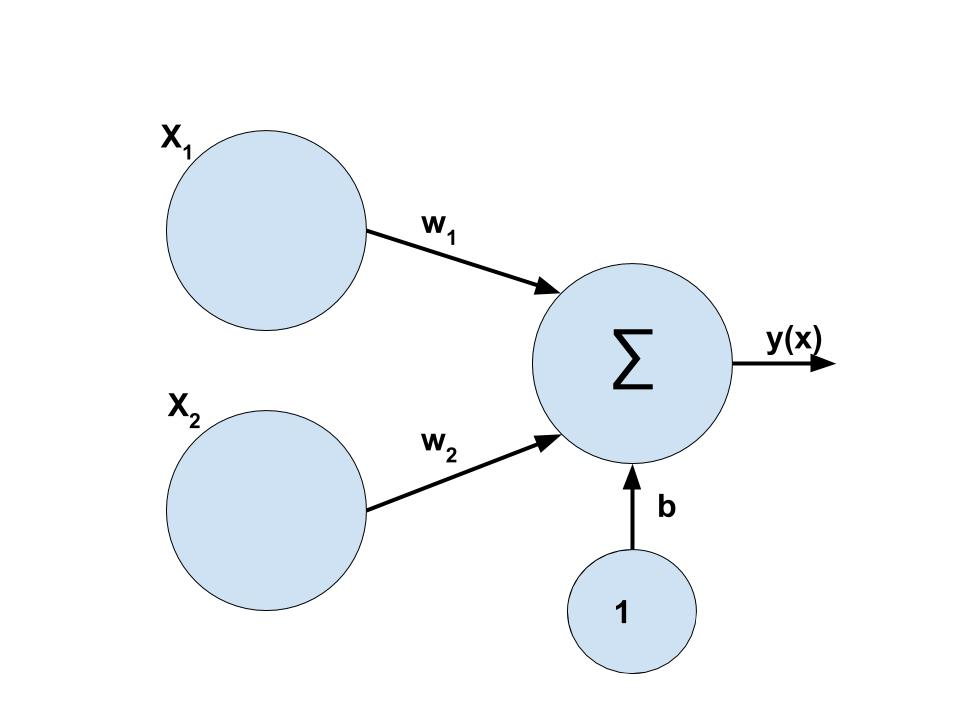
\includegraphics[width=0.55\textwidth]{images_miscelaneus/neurona_sencilla.jpg}
\caption{Simplest neural network architecture.} \label{fig:neuronasencilla}
\end{figure}

The simplest example of a neural network is formed by two inputs neurons and a output neuron as it is shown in figure \ref{fig:neuronasencilla}in which \textit{$W=[w_1,w_2]$} are refered to the weights assigned to each neuron. The \textit{b} value is refered to the bias term. \textit{$X=[x_{1},x_{2}]$} are the input of the network architecture and \textit{y(x)} the output. The output is predetermined by the equation \ref{eq:ecuation_neuronasencilla}. So, the output would depend on the input, weights and bias sand the activation function (or transfer function) \textit{F} \cite{krose}. \\

%Ecuacion salida neurona
			\begin{equation}
			y(x)=F(\sum_{i=1}^{2} (w_{i}*x_{i} + b) )
			\label{eq:ecuation_neuronasencilla}
			\end{equation}\\

Due to activation function, the output of the neuron would change if the input is bigger than a some threshold. This threshold is defined by the own activation function. There are various functions that are used: sigmoid function, Heaviside function, Fermi function or hyperbolic tangent among others. In figure \ref{fig:activation_function} (which has been obtained from \cite{BINN}) the mentioned function are shown and the output would be 0 or 1 values if the function is sigmoid or Fermi and the output would be -1 or 1 if the function is an hyperbolic tangent. \\

\begin{figure}[htb]
\centering
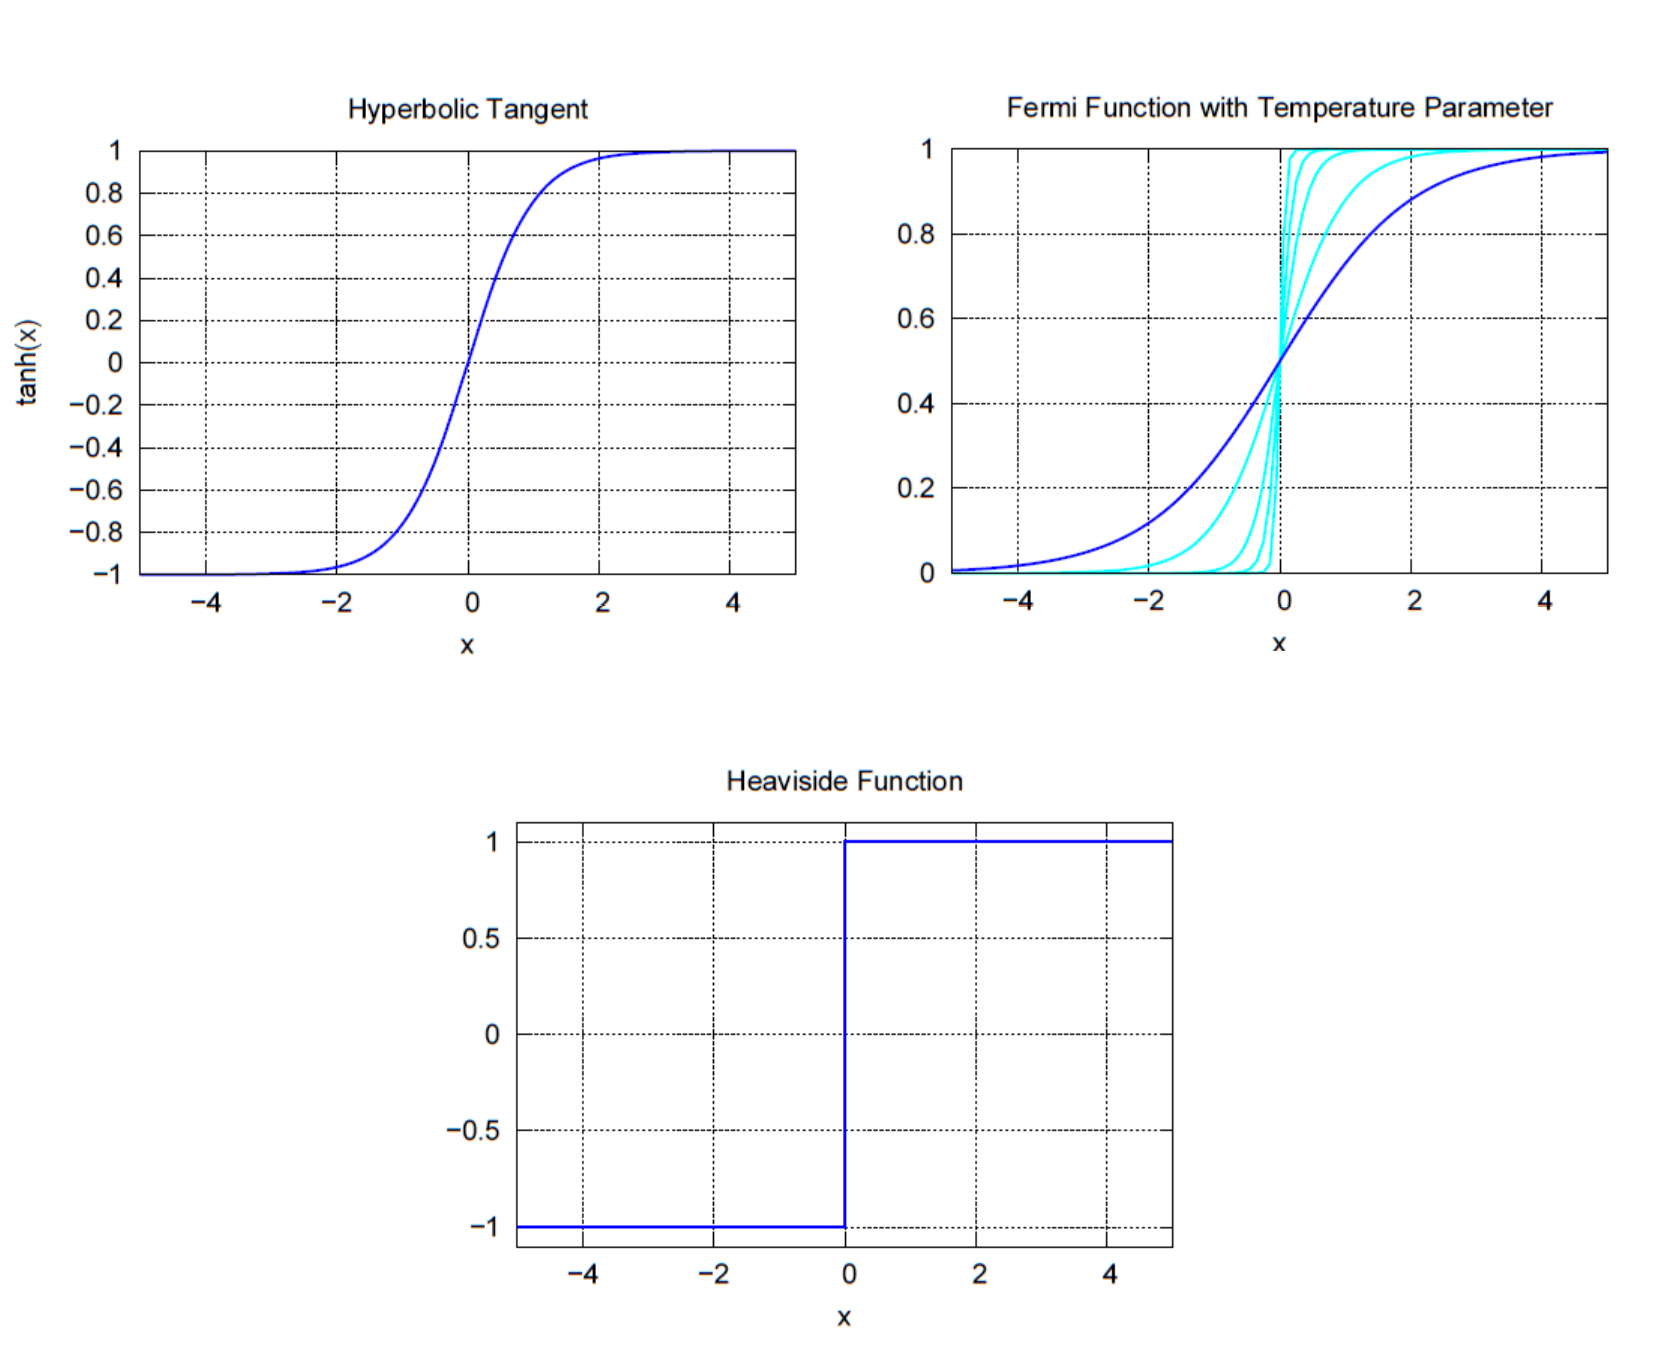
\includegraphics[width=0.55\textwidth]{images_miscelaneus/activation_function.PNG}
\caption{Different activation functions. Image obtained from \cite{BINN}} \label{fig:activation_function}
\end{figure}

\subsubsection{Analogies between ANN and Biological Neural Networks}
Analogies between Artificial and Biological Neural networks could be found (if both basic theory is known) because the first one (artificial NN) are based in the second one. It is easy to see that biological neurons correspond to artificial neurons. But the cell body correspond with transference function. The output to others neurons would correspond to the axon and synapses with weights and bias. The soma would correspond with the transfer function. Those analogies are summarized in table \ref{table:Analogias}. Artificial neural networks are just inspired in Biological neural networks, that both work in a different (although inspired) way must be made clear.\\

\begin{table}[htb]
\centering
\begin{tabular}{|c|c|}
\hline
\rowcolor[HTML]{ECF4FF} \textbf{Artificial Neural Component} & \textbf{Analogy}        \\ \hline
Neuron Artificial Neuron                        & Biological Neuron       \\
Transfer function                & Soma \\
Connexion between Artificial neurons               & Axón                     \\
Weight                                     & Synapses                 \\ \hline
\end{tabular}  \caption{Analogies between artificial neural networks and biological neural networks} \label{table:Analogias}
\end{table}

\subsubsection{Learning}
Neuronal networks are able to learn features from the input to classify or just extract features of the input data. In order to know how to get the desired output, a learning process is needed. The learning process what really do is modifying weights and bias values for each layer with the purpose of getting a better output \cite{NNDesign}.\\

There are three main different learning procedures that defined following \cite{NNDesign,Duda}:
\begin{description}[noitemsep,topsep=8pt,parsep=0pt,partopsep=20pt]
	\item \textbf{Supervised Learning:} the input training data is given with its target (correct result of its corresponding sample), that means that the train samples has associated the desired output. The learning consist in adjust the weights and bias until the output of the network is the same or the closest value as the target.
	\item \textbf{Reinforcement Learning:} in the training, the correct target is not provided, but just a grade is given to the network.
	\item \textbf{Unsupervised Learning:} there is not help in the training, no target and no grade, just the input data. The networks learn to cluster the input data and the weights and bias changes in function of the bias.
\end{description}

All the learning procedures in neural networks have in common the modification of weights ans bias to learn and obtain the desired output, so the error at the output is minimized. The most useful learning procedure is the supervised learning.\\

The gradient descend procedure is an algorithm whose goal is minimize the error of a function \textit{J}.\textit{J(a)} would be the minimum if \textit{a} is the solution. To get the solution the gradient of \textit{J} ($\nabla J(a)$) is calculated for each value of \textit{a}: $\nabla J(a(1))$ is obtained and \textit{a(2)} is obtained moving some distance from \textit{a(2)}, in steps called \textit{learning rate $\eta$}, in direction of the negative gradient. The \textit{a(k+1)} value would be: \cite{Duda}.\\

\begin{equation}
a(k+1) = a(k) - \eta (k) \nabla J(a(k))
\end{equation}

One of the most used supervised techniques of neural network learning is the back-propagation, this learning rule is based in the gradient descend. In general, this rule, from a randomize initialization of weights, the error would be minimized changing the weights in the direction of the gradient descend:

\begin{equation}
\delta w = -\eta\frac{\partial J}{\partial w}
\end{equation}

Being $\frac{\partial J}{\partial w}$ The gradient of \textit{J} in function of weights \textit{w}.

The error is calculated as defined in equation \ref{eq:error_bb}

%Ecuacion error 1
\begin{equation}
E=\sum_{p}E^p = \frac{1}{2}\sum_{p}(\delta^p- y^p)^2
\end{equation} \label{eq:error_bb}

The error is backpropagated to the last layers until the first layer, modifying the weights to balance the error proportionally to the gradient of the error function. This is called the chain rule or the delta rule \cite{Duda, BINN, krose}. The backpropagation equation is defined below\\

%Ecuacion backpropagation 1
			\begin{equation}
			\Delta_{p}W_{jk}=ºeta \delta _{k}^{p}y_{j}^{p}
			\label{eq:ecuation_back1}
			\end{equation}\\

Being  \textit{k} the unit which receives the input and \textit{j} the output.\\

There are three useful training protocols depending on how training set is used:
\begin{description}[noitemsep,topsep=8pt,parsep=0pt,partopsep=20pt]
	\item \textbf{Stochastic training:} Samples are choosen randomly and for each sample, weights are updated.
	 \item \textbf{Batch training:} All training samples are used to the learning process.
	 \item \textbf{on-line training:} There is no memory, as the same time as samples are received, they are used once to train.
\end{description}


\subsubsection{Type of Layers}
The layers that conforms the networks could be different depending on the mathematical operation. The most common used layers are described below:
\begin{description}[noitemsep,topsep=8pt,parsep=0pt,partopsep=20pt]
	\item \textbf{Convolutional layer:} In this type of layers, the convolution operator is processed at the input. Weights are the applying filters and the output are the features or characteristics useful to extract the information of the image. In one convolutional layer, there could be used as many filters are user defines.
	\item \textbf{Pooling Layer:} In this layer, the dimensionality is reduced. The most important information is preserved. It is usually used at the output of the convolutional to resume its out \cite{Doorn}. The most used pooling layer is the max-pooling layer, the maximum values are saved.
	%\item \textbf{No-linearity layer:} Esta capa consta de una función sigmoide punto tanh() aplicado a la entrada de la capa. Sin embargo, en las implementaciones recientes, se han utilizado otras no linealidades más sofisticadas \cite{Lecum3, Doorn}.
	\item \textbf{Normalization layer:} This layer normalize the activities of the neurons, because of that the processing time could be reducing during training or testing. There are two types of normalization layer: Local Response Normalization (LRN) and Batch Normalization.
	\item \textbf{Dropout layer:} The ouput of a network could rely on the output of an spefici neurons being this a overfitting cause. To prevent it, during training, some neurons are 'turn off´ setting its value to 0. In this way, neurons are more adaptative. Dropout is a spefic layer that manage this. In stead of \textit{eliminate} neurons, if it is possible that weights are put to 0. In this case, the layer would be \textbf{``DropConnect''} \cite{Doorn}.
	\item  \textbf{Fully-connected layer:} Fully connected layer is vector in which the input is connected to each nenuron that conforms this layer. This layer is the high-level reasoning layer so, it is used before the classification.
\end{description}

One neural network is defined by its type of layers and the number of neurons, also, there are parameters that also affect to the behaviour of the network (learning rate,...)\cite{Lecum2}.\\

%\subsection{Type of Networks}

%\begin{description}[noitemsep,topsep=8pt,parsep=0pt,partopsep=20pt]
%	\item \textbf{Siamese:}
%	\item \textbf{Convolutional:}
%	\item \textbf{Recurrent:}
%\end{description}

\section{Convolutional Neural Network (CNN)}
Convolutional neural network are a determinate typology of neural network, CNN are inspired in how the visual cortex of a cat works \cite{Doorn}. This type of neural networks are (usually) used with images at the input of the network.\\

Convolutional neural network has been used successfully in recognition and classification task includying document and object recognition, face detection, robotics navegation... \cite{Lecum2, Lecum3}.\\
